
\documentclass{scrartcl} % KOMA Dokumentenklasse mit DIN-Papier als Standard
\usepackage[a4paper]{geometry} % Paket zur flexiblen Anpassung des Seitenlayouts
\savegeometry{default}
\usepackage[autooneside=false]{scrlayer-scrpage} % Paket zur flexiblen Anpassung der Kopf- und Fußzeilen
%
%\usepackage[tocindentauto]{tocstyle} % Paket zur flexiblen Anpassung der Formatierung des Inhaltsverzeichnisses (wird hier nur benötigt, weil einmalig die Nummerierung auf römische Zahlen umgestellt wurde)
 %\usetocstyle{KOMAlike}
%
\usepackage[english]{babel} % Sprachenpaket zur Anpassung der Standardausgaben von bestimmten Schlüsselwörtern und Aktivierung der deutschen Silbentrennung
%
\usepackage{miller}%to intuitively display miller indices%

\usepackage{parskip} %gets rid of hbox warning - just add empty lines to imply linebreaks

\usepackage[utf8]{inputenc} % Kodierungspaket zur Festlegung, wie die eingegebenen Zeichen (Code hier im Dokument) interpretiert werden sollen
%
\usepackage{csquotes}

\usepackage[T1]{fontenc} % Kodierungspaket zur Festlegung, wie die ausgegebenen Zeichen (Buchstaben im PDF-Dokument) implementiert werden sollen
%
\usepackage{lipsum} % Paket zur Einbindung von lateinischen Blindtexten
%
\usepackage{multicol} % Paket zur flexiblen Erstellung mehrspaltiger Texte und zum Zusammenfassen von Spalten in Tabellen
%
\usepackage{ragged2e} % Paket zur Verbesserung der Darstellung von linksbündigem, rechtsbündigem und zentriertem Text (erlaubt Silbentrennung)
%
\usepackage{quoting} % Paket zur ansprechenden Darstellung von Zitaten
%
\usepackage[marginal,norule]{footmisc} % Paket zur flexiblen Anpassung der Formatierung von Fußnoten
%
\usepackage{listings} % Paket zur vereinfachten Einbindung und zur ansprechenden Darstellung von Code in beliebigen Programmiersprachen
%
\usepackage[section, below]{placeins}
%\usepackage[section]{placeins}
%
%
\usepackage{microtype} % Paket zur Verbesserung der Mikro-Typographie durch Anpassung von Zeilenenden und sinnvollen Reduzierung von Silbentrennungen
\usepackage{lmodern} % Schriftenpaket für Latin Modern Schriften (beliebig skalierbare, richtig implementierte Vektorschriften)
%\renewcommand{\rmdefault}{lmss} %to use sans serif by default
\usepackage{textcomp} % Paket zur Erweiterung von verfügbaren Sonderzeichen (Copyright, Trademark, ...)
%
\usepackage{textgreek} %to use greek letters in text
%
\usepackage{amsmath} % Extrem umfassendes Mathematik-Paket der American Math Society
% allow for wider matrices
\newcommand{\tens}[1]{\boldsymbol{\mathsf{#1}}}
\setcounter{MaxMatrixCols}{20}
\usepackage{mathtools} % Erweiterung des amsmath-Pakets (enthält amsmath-Paket)
% Ergänzungen für Mathe:
\DeclarePairedDelimiter\abs{\lvert}{\rvert}%
\DeclarePairedDelimiter\norm{\lVert}{\rVert}%
%
%
% Anpassung von Klammern 
% Swap the definition of \abs* and \norm*, so that \abs
% and \norm resizes the size of the brackets, and the 
% starred version does not.
\makeatletter
\let\oldabs\abs
\def\abs{\@ifstar{\oldabs}{\oldabs*}}
%
\let\oldnorm\norm
\def\norm{\@ifstar{\oldnorm}{\oldnorm*}}
\makeatother
%
%
\usepackage{amsfonts} % Schriftenpaket der American Math Society zur Erweiterung der Schriften in Mathe-Umgebungen
%
\usepackage{amssymb} % Paket zur Erweiterung der verfügbaren Mathe-Symbole
%
\usepackage{MnSymbol} % Paket zur Erweiterung der verfügbaren Mathe-Symbole
%
\usepackage{graphicx} % Paket zur vereinfachten und flexiblen Einbindung von Grafiken (jpg, png, pdf)
%
\usepackage{pdfpages} % Paket zur vereinfachten und flexiblen Einbindung von mehrseitigen PDFs
%
\usepackage{chemformula} %Paket für chem. Formeln e.g. with \ce or \ch and stuff in brackets
%
\usepackage{xcolor} % Farbenpaket zur vereinfachten Einbindung und Anpassung von Farben
%
\usepackage{booktabs} % Paket zur Verbesserung der Darstellung von horizontalen Linien in Tabellen
%
\usepackage{multirow} % Paket zum Zusammenfassen von Zeilen in Tabellen
%
\usepackage{tikz} % Paket zur Erstellung von ansprechenden und anspruchsvollen Zeichnungen innerhalb von LaTeX
%\usepackage{pgfplots} % Paket zur Erstellung von ansprechenden und anspruchsvollen Plots innerhalb von LaTeX
%
\usepackage[style=nature, backend=biber]{biblatex} % Paket zur vereinfachten und automatisierten Erstellung eines Literaturverzeichnisses aus einer externen Datenbank

%
\usepackage{xparse} % Paket zur Erweiterung der Funktionalitäten bei der Definition von neuen Befehlen und Umgebungen
%
\usepackage{hyperref} % Paket zur Erstellung und Anpassung von anklickbaren, intelligenten Querverweisen innerhalb des Dokuments und Hyperlinks (Weblinks, Maillinks, Filelinks)
%
%
%
%
% Einstellungen für das Dokument:
%
 \KOMAoptions{headsepline, footsepline}
 \setkomafont{headsepline}{\color{gray}}
 \setkomafont{footsepline}{\color{gray}}
 \setkomafont{pagehead}{\scshape}
 \setkomafont{pagefoot}{} %\bfseries
 \automark[subsection]{section}
 \lohead{}
 \cohead{\rightmark}
 \rohead{}
 \lofoot{}
 \cofoot{\pagemark}
 \rofoot{}
%
%
\definecolor{meinSchwarz} {RGB} {0,0,0}
%
\hypersetup{linktoc = all, colorlinks ,  citecolor = meinSchwarz , linkcolor = meinSchwarz, urlcolor  = meinSchwarz , filecolor = meinSchwarz }
%
%\addto\extrasngerman{\def\figureautorefname{Abb.}}
%
\setlength{\parindent}{0pt}
\setlength{\parskip}{0.5\baselineskip plus 0.2\baselineskip minus 0.1\baselineskip}
\linespread{1.25}
%
\newcommand{\degcel}{\,\textcelsius{} }
%
% Angaben zu Variablen
\graphicspath{{graphics}}
\bibliography{ddd_bib}
%

\begin{document}

%
\begin{titlepage}
\begin{center}

\includegraphics[width=0.5\textwidth]{graphics/FAU_TechFak_EN_H_black.eps}

\LARGE Department Materials Science

\Large WW8: Materials Simulation

\LARGE \textbf{Practical: Discrete Dislocation Dynamics simulation}



\vfil
\Large Leon Pyka (22030137)



\Large \textbf{Supervision: }
\end{center}

\thispagestyle{empty}
%
\end{titlepage}
%

\setcounter{page}{1}

\tableofcontents
\newpage

\section{Introduction}
The topic of this practical is to get an introduction into \textit{discrete dislocation dynamic} (DDD)  simulations. In the course of the following exercises the open-source software \textit{microMegas} (mM) is utilized \cite{devincre2011}.  

\subsection{General Aspects of Dislocation Dynamics} 

As it is common for DDD simulation, three steps are carried out to model the dynamics of the dislocations:

\begin{enumerate}
	\item calculate the stress field 
	\item calculate the Forces acting on the dislocation line segments (according to eq. \ref{eq:peach-koehler} - the Peach-Köhler equation)
	\item moving the line segments accordingly - the velocities are calculated according to eq. \ref{eq:vleocities_mobility_func} and are moved following forward Euler (eq. \ref{eq:forward_euler})
\end{enumerate}

\begin{equation}
	F = (\sigma_{ext}+\sigma_{int}) \mathbf{b}l  \label{eq:peach-koehler}
\end{equation}

The Peach-Köhler Equation (eq. \ref{eq:peach-koehler}) takes into account internal- \( \sigma_{int} \) and external stresses  \( \sigma_{ext} \) acting on dislocation segments of vector \(l\) with a burgers vector of \( \mathbf{b}\). In mM (and similar frameworks) \( \sigma_{ext}\) is imposed on the system as a parameter. 

\begin{subequations}
	\begin{align}
		v =& M(F) \label{eq:vleocities_mobility_func} \\
		r(t+\Delta t) =& r(t) + v(t)\Delta t \label{eq:forward_euler}
	\end{align}
\end{subequations}

The velocities of the segments are a functional of the mobility function \(M(F)\) depending on the individual forces, the material and the orientation of the segment. The segments positions are calculated as a result of the the application of the forward Euler scheme - eq. \ref{eq:forward_euler}. The new position \( r(t+ \Delta t)\) after a time step of \(\Delta t\) is calculated as the position \(r(t)\) being moved according to its velocity \(v(t)\). For forward Euler being applicable we assume quasi-static deformation. 

As a result of the forces imposed on a dislocation, the dislocation might curve. In mM this is achieved by cutting the curved line into several segments. These segments are discretized as depicted in fig. \ref{fig:schematic_segments_dislocs}. The choice to include 8 slip systems in mM was made as trade-off - balancing the increasing complexity with the best representation of the curved dislocation \cite{devincre2011}.

\begin{figure}[htb]
	\centering
	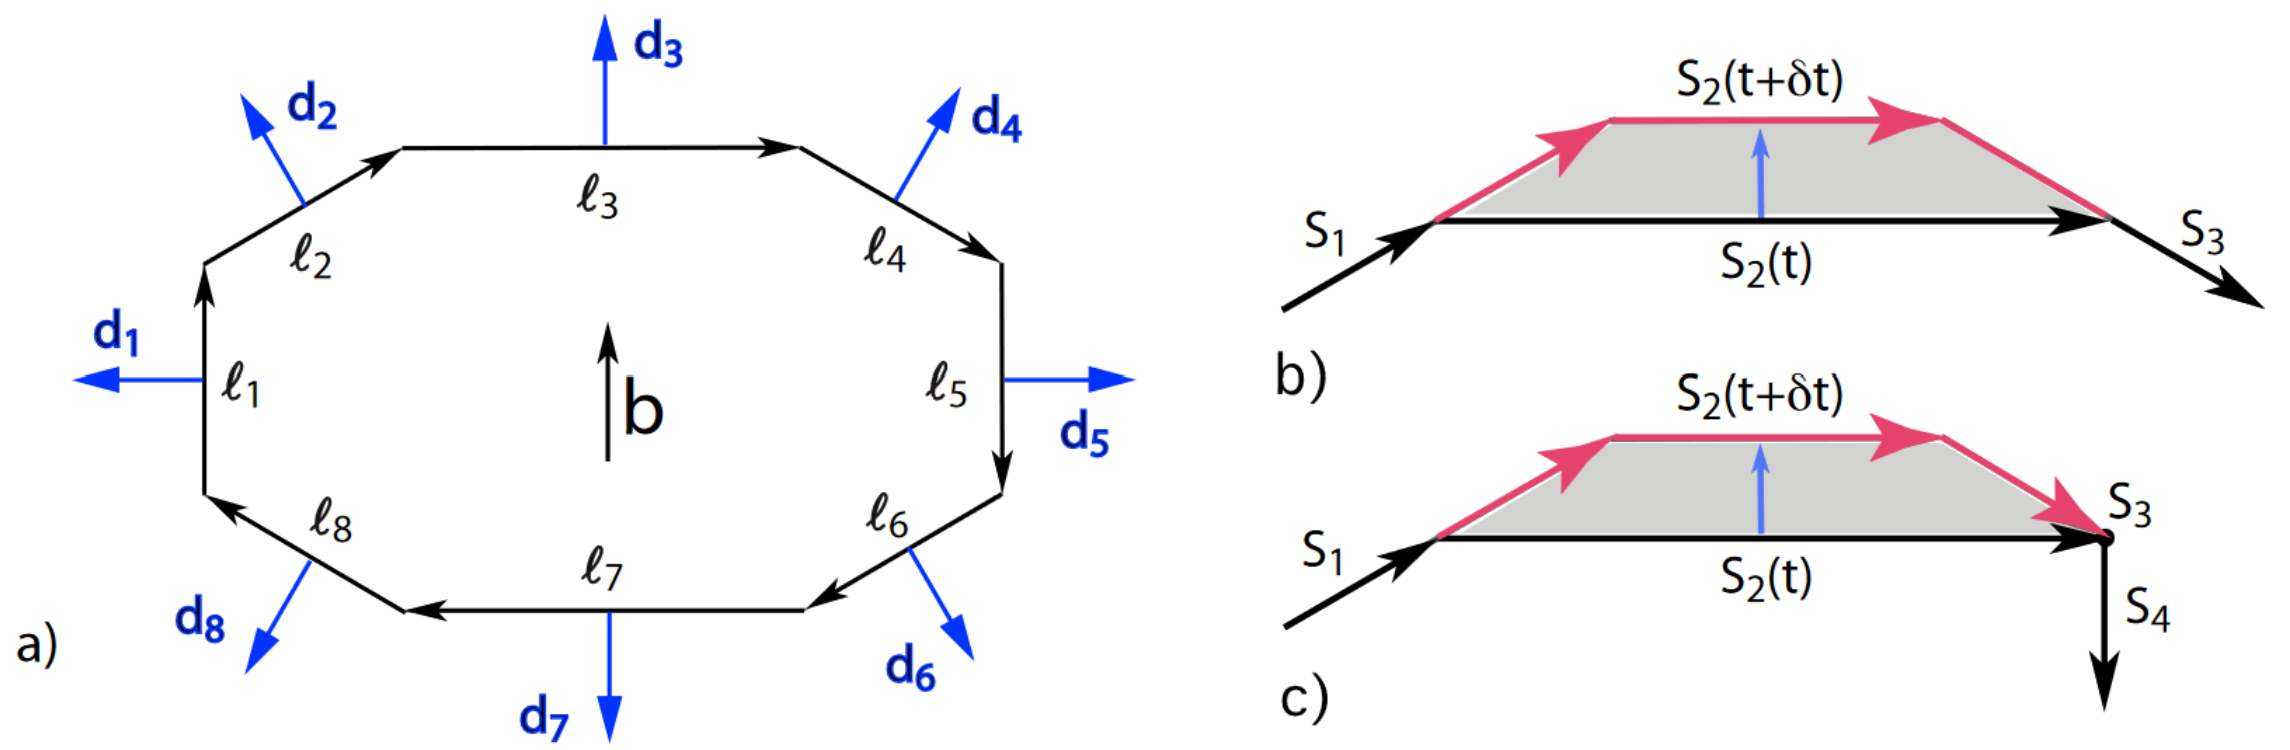
\includegraphics[width=\textwidth]{schematic_discretized_disloc_lines.png}
	\label{fig:schematic_segments_dislocs}
	\caption{a) Schematic representation of the elementary vectors used per slip system to discretize dislocation lines in mMs. The vectors \(l_{1-8}\)(in black), are used for the definition of the segments directions and the vectors \(\mathbf{d}_{1-8}\)(in blue) for the corresponding displacement directions. b) and c) Geometrical procedures for the displacement of a segment and its length variation. b) The trapezoidal area swept by segment S2 during a time step \(\Delta t\)(in grey) produces and increment of plastic shear.This procedure accounts for the direction of the two neighbouring segments. c) Before the displacement, a local rule for connections imposes the presence of a "pivotal segment" \(S_{3}\) (segment of zero length) between segments \(S_{2}\) and \(S_{4}\) reproduced from \cite{devincre2011}.}
\end{figure}

\FloatBarrier
\subsection{Frank-Read Source}

The Frank-Read source is going to be in the main focus of these exercises. A Frank-Read source is a dislocation segment that is pinned at two points. The force acting on it is generally the Peach-Köhler equation (eq.~\ref{eq:peach-koehler}), where the resolved shear stress \(\tau\) is acting on the segment:
\begin{equation}
	F =  \cdot \tau \mathbf{b}l
\end{equation} 

Above a certain critical shear stress \(\tau_{crit}\) the dislocation segment is becoming an infinite source for dislocation loops (see fig. \ref{fig:frank-read-scheme}). The two folders 

\begin{figure}[htb]
	\centering
	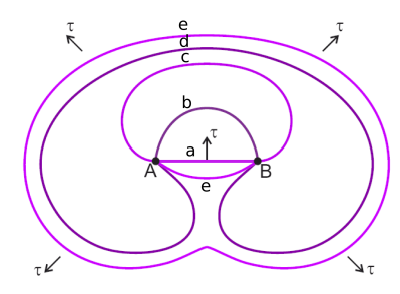
\includegraphics[width=\textwidth]{schematics_frank_read.png}
	\caption{ Activation of a Frank-Read source: Dislocation segment (a) is pinned at point A
		and B. Under the applied shear stress τ it starts to bow out (b) till it reaches
		its critical configuration (c), and then expands through its unstable state (d) till
		self-anihilates to a dislocation loop and a new FR segment (e) reproduced from \cite{zaiser}.}
	\label{fig:frank-read-scheme}
\end{figure}

The bow out stress given by Hirth ( \cite{anderson2017}, P. 752):

\begin{equation}
	b\tau_{crit} = \frac{\mu b^{2}}{4\pi r(1-\nu)} \biggl\{ \biggl[\ 1- \frac{\nu}{2}(3-4\cos^{2}\beta) \biggr]\ \ln \frac{L}{\rho} -1 + \frac{\nu}{2} \biggr\} \label{eq:tau_crit}
\end{equation}

for the common case of \( L =1000\rho \) is simplified to: 

\begin{equation}
	\tau_{crit} = \alpha \frac{\mu b}{L}
\end{equation}

with \(\alpha\) being 0.5 for pure edge dislocations and 1.5 for pure screw dislocations \cite{zaiser}. 

\section{Simulation Setup (Task 1)}
The first Task deals with setting up a simulation of a pinned edge dislocation in mM. It acts as both an introduction the the software and an initial state for the following tasks.

\subsection{Installing and Getting to Know The Software (Task 1.1 - 1.4)}
In the first Task the required software is installed from the \href{http://zig.onera.fr/mm_home_page/}{microMegas Homepage}. When running on a linux machine, virtual machine or WSL one can go to the \code{\textbackslash bin} folder and ron \code{make all} to compile the source files. The folder in which most work are done are \code{\textbackslash in} and \code{\textbackslash out}. Under \code{\textbackslash in} the input files are defined in \code{input.dd}:

\begin{enumerate}
	\item material specific data (e.g. Shear Modulus, Burgers Vector Norm, slip planes, slip directions)
	\item simulation specific data (e.g. initial stress, stress increment, time step, echelle - size of elementary screw vector)
	\item data defining the dislocation segments (position, composition, pinning)
\end{enumerate}

To run the simulation we run \code{.bin\textbackslash gmm}(for interactive mode with graphical interface - see fig. \ref{fig:mm_gui}). The output can be visualized in the \code{\textbackslash out} folder using plotting the data saved to the \code{graph.txt} file.

\begin{figure}[htb]
	\centering
	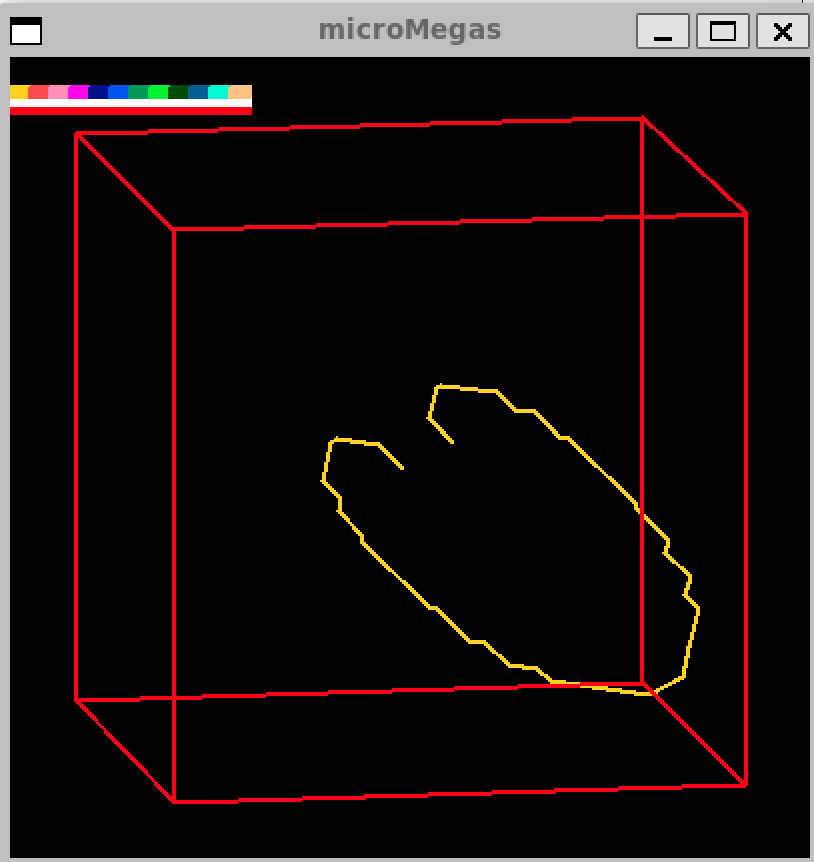
\includegraphics[width=0.5\textwidth]{mM_gui_eg.png}
	\caption{GUI of mM}
	\label{fig:mm_gui}
\end{figure}

\subsection{Defining the Simulation Box (Task 1.5)}

Since the documentation of mM is not very clear on how the input is interpreted, it has to be deduced which input has an effect on the output. The \code{echelle} value in the \code{CuSeg} file seems to have an effect on the reference scale of the simulation as depicted in the \code{BVD.CFC} file. If we leave the initial value of \code{echelle} at 13.5 the reference scale is \(1.2183007689602674'10^{-9}\). Following the notes given in the respective README files and assuming that this value is given in units of meter, we can derive, that in the file defining our dislocation segments, we need to use a value of 2464 to have approximately \(3~\mu m\)5as the box dimensions.

\subsection{Defining the Pinned Edge Dislocation (Task 1.6)} \label{sec:task1_6}

For the pinned edge dislocation we define an input file \code{Seg\_Pinned\_Edge} as follows:
\begin{tabular}{l}
	\code{1 1 1 1 1 1 1 1 1 1 1 1} \\
	\code{1} \\
	\code{2464 2464 2464} \\
	\code{1 1200 1200 1200 80 3 0 0 0 0 F 0 0} \\
\end{tabular}

The first line defines which slip-systems are active (here all), the second is the number of dislocation segments the third defines the box size as a multiple of BVD units. The third line defines the dislocation as follows: column 1 - The segment index, column 2 - x coordinate of the segment origin, column 3 - y coordinate of the segment origin, column 4 - y coordinate of the segment origin, column 5 - length of the segment in BVD vector unit, column 6 - index of the BVD vector parallel to the segment direction, column 7 - first neighbor segment at the origin of the segment (zero for pining point), column 8 - first non zero length neighbor segment at the origin (idem), column 9 - first neighbor segment at the extremity side (idem), column 10 - first non zero length neighbor segment at the extremity side (idem), column 11 - Flag for junction segment, column 12 - index of the binome segment use to form a junction, column 13- Flag for screw segment in cross-slip state (blocked at the intersection of different glide planes). This is stated as a comment in an initial file, although it is not explicitly stated, what "idem" means. 
When running the simulation without an applied stress the \code{graph.txt} output shows a value for the dislocation density that is 4 times the expected value. For these reasons the number of segments previously chosen in section \ref{sec:task1_6} is readjusted to be 20 instead of 80. This now leads to a dislocation density of \( \rho = 0.44127*10^{10}~\frac{1}{m^{2}}\) that is a segment length of \(L \approx 119~nm\).

\subsection{Estimation of Critical Activation Stress (Task 1.7)}
The critical shear stress \(\tau_{crit}\) can be estimated using \ref{eq:tau_crit}. With \(\alpha = 0.5\), \(\mu = 25.0~MPa\), \(b = 2.5525~\AA\) and a length of \(L \approx 119~nm \). Resulting in an estimate value of \(\tau_{crit} = 45.0~MPa\). \\


%\listoffigures
\printbibliography

\end{document}
